\paragraph*{Structural reference for attention interpretation.}
Figure~\ref{fig:attn-priors} distinguishes the factory adjacency, hop proximity and semantic similarity used as structural references from the learned weights examined in Section~5.3. The visualization is exported from the supplementary \texttt{dense\_i1\_mix} checkpoint family, rather than the retained \texttt{dense\_i1} checkpoints. For readability, the matrices display the 20 non-buffer resources---seven machines/workbenches, four gantries, five workers and four AGVs---while retaining the corresponding entries from the full 38-node model graph. The graph and similarity matrices provide the reference against which attention redistribution is interpreted; they are not estimates of learned resource importance.
\zhpara{图~\ref{fig:attn-priors}区分工厂邻接、跳数接近度和语义相似度三类结构参照，为第5.3节的注意力分析提供依据。该可视化导出自补充的 \texttt{dense\_i1\_mix} checkpoint 系列，并非主结果中保留的 \texttt{dense\_i1} checkpoint。为提高可读性，矩阵显示完整三十八节点模型图中二十个非缓冲区资源，即七个机器或工作台、四个龙门、五名工人和四台 AGV，并省略十八个缓冲区行列。结构矩阵用于理解注意力的分配基础，不应直接解释为模型学到的资源重要性。}
\begin{figure*}[p]
\centering
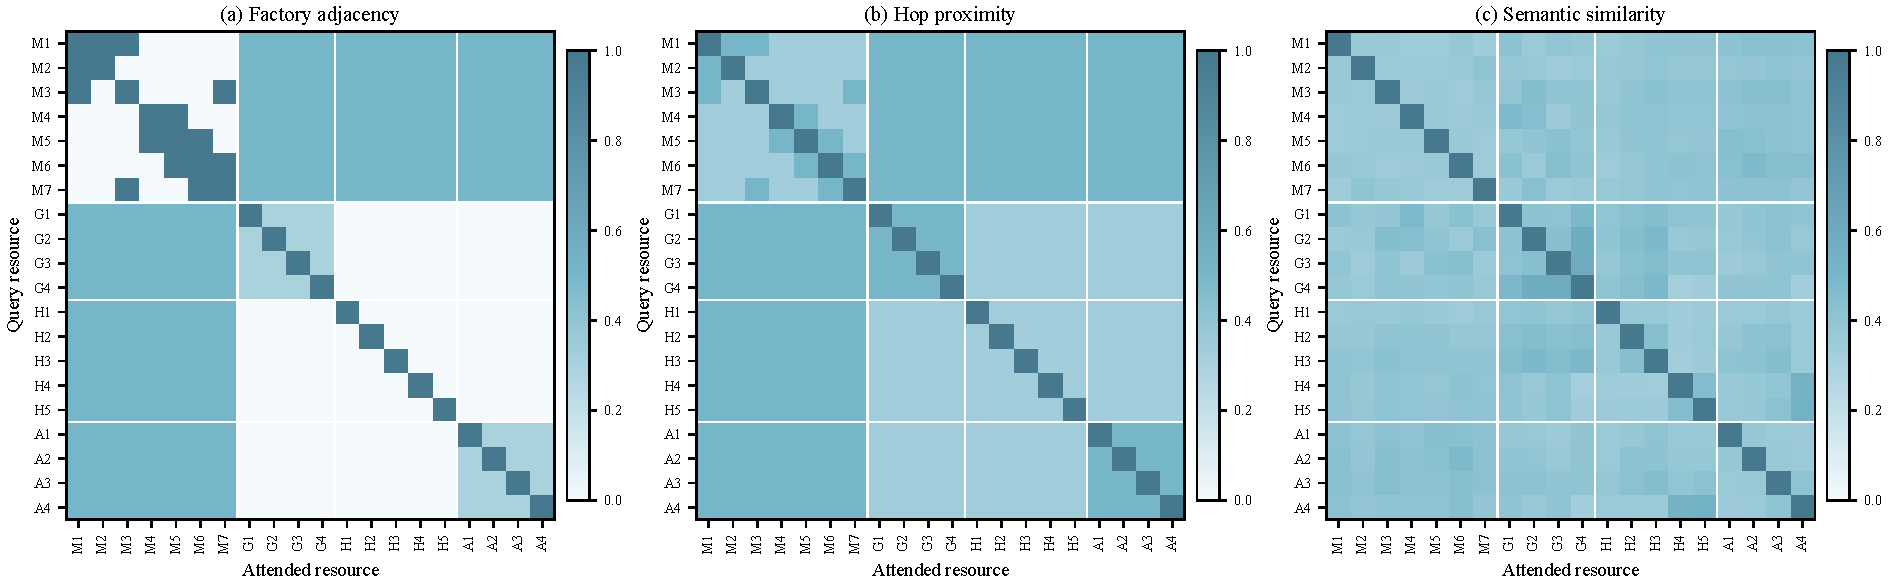
\includegraphics[width=0.98\textwidth,height=0.78\textheight,keepaspectratio]{figures/attention_heatmaps/fig01_graph_priors.pdf}
\caption{Structural reference matrices for the 20 displayed non-buffer resources: (a) factory adjacency, (b) hop proximity and (c) semantic similarity. M/G/H/A denote machine, gantry, human and AGV; rows are query resources and columns attended resources. The matrices retain entries from the full 38-node model graph. Mixed-disturbance supplementary analysis (\texttt{dense\_i1\_mix}, seed 42); not the retained \texttt{dense\_i1} evaluation.}
\label{fig:attn-priors}
\end{figure*}
